%%%%%%%%%%%%%%%%%%%%%%%%%%%%%%%%%%%%%%%%%
% Stylish Article
% LaTeX Template
% Version 2.2 (2020-10-22)
%
% This template has been downloaded from:
% http://www.LaTeXTemplates.com
%
% Original author:
% Mathias Legrand (legrand.mathias@gmail.com) 
% With extensive modifications by:
% Vel (vel@latextemplates.com)
%
% License:
% CC BY-NC-SA 3.0 (http://creativecommons.org/licenses/by-nc-sa/3.0/)
%
%%%%%%%%%%%%%%%%%%%%%%%%%%%%%%%%%%%%%%%%%

%----------------------------------------------------------------------------------------
%	PACKAGES AND OTHER DOCUMENT CONFIGURATIONS
%----------------------------------------------------------------------------------------

\documentclass[fleqn,10pt,ngerman]{SelfArx} % Document font size and equations flushed left

\usepackage{babel} % Specify a different language here - German in this case

\usepackage{csquotes} % used for German quotes

\usepackage{lipsum} % Required to insert dummy text. To be removed otherwise

\usepackage{subcaption} % used for subfigures

\usepackage{tikz} % used for tikz figures

\usepackage{pgfplots} % used for pgfplots

\usepackage[%
    backend=biber,  % use bibtex as backend
    urldate=iso,    % use iso date format for urls
    seconds=true,   % display seconds in time stamps, needed for urldate
    natbib=true,    % enable natbib compatibility
    % style=ieee,     % use ieee style
    sorting=none    % sort by appearance in document
]{biblatex} % bibliography

\addbibresource{literatur.bib}

%----------------------------------------------------------------------------------------
%	COLUMNS
%----------------------------------------------------------------------------------------

\setlength{\columnsep}{0.55cm} % Distance between the two columns of text
\setlength{\fboxrule}{0.75pt} % Width of the border around the abstract

\setlength\emergencystretch\textwidth % prevent overfull lines

%----------------------------------------------------------------------------------------
%	COLORS
%----------------------------------------------------------------------------------------

\definecolor{color1}{RGB}{0,0,90} % Color of the article title and sections
\definecolor{color2}{RGB}{0,20,20} % Color of the boxes behind the abstract and headings

%----------------------------------------------------------------------------------------
%	HYPERLINKS
%----------------------------------------------------------------------------------------

\usepackage{hyperref} % Required for hyperlinks

\hypersetup{
	hidelinks,
	colorlinks,
	breaklinks=true,
	urlcolor=color2,
	citecolor=color1,
	linkcolor=color1,
	bookmarksopen=false,
	pdftitle={Title},
	pdfauthor={Author},
}

%----------------------------------------------------------------------------------------
%	ARTICLE INFORMATION
%----------------------------------------------------------------------------------------

\JournalInfo{Praktikum Computergrafik SoSe 2023} % Journal information
\Archive{M. Sc. Hendrik Brückler, Prof. Dr. Marcel Campen} % Additional notes (e.g. copyright, DOI, review/research article)

% \PaperTitle{Erzeugung von Mikrokosmen mittels Lenia-Algorithmus und Fraktalen mittels Ray-Marching} % Article title
\PaperTitle{Visualisierung von Mikrokosmen und Fraktalen mit dem Lenia-Algorithmus und dem Ray-Marching-Verfahren} % Article title

\Authors{\phantom{Author}} % Authors
% \affiliation{\textsuperscript{1}\textit{Department of Biology, University of Examples, London, United Kingdom}} % Author affiliation
% \affiliation{\textsuperscript{2}\textit{Department of Chemistry, University of Examples, London, United Kingdom}} % Author affiliation
% \affiliation{*\textbf{Corresponding author}: john@smith.com} % Corresponding author

% \newcommand{\SeminarKind}{Programmierpraktikum}
\newcommand{\SeminarTitle}{Praktikum Computergrafik}
\newcommand{\SeminarTerm}{Sommersemester 2023}

% \Keywords{Keyword1 --- Keyword2 --- Keyword3} % Keywords - if you don't want any simply remove all the text between the curly brackets
\newcommand{\keywordname}{Keywords} % Defines the keywords heading name

%----------------------------------------------------------------------------------------
%	ABSTRACT
%----------------------------------------------------------------------------------------

% \Abstract{Lorem ipsum dolor sit amet, consectetuer adipiscing elit. Ut purus elit, vestibulum ut, placerat ac, adipiscing vitae, felis. Curabitur dictum gravida mauris. Nam arcu libero, nonummy eget, consectetuer id, vulputate a, magna. Donec vehicula augue eu neque. Pellentesque habitant morbi tristique senectus et netus et malesuada fames ac turpis egestas. Mauris ut leo. Cras viverra metus rhoncus sem. Nulla et lectus vestibulum urna fringilla ultrices. Phasellus eu tellus sit amet tortor gravida placerat. Integer sapien est, iaculis in, pretium quis, viverra ac, nunc. Praesent eget sem vel leo ultrices bibendum. Aenean faucibus. Morbi dolor nulla, malesuada eu, pulvinar at, mollis ac, nulla. Curabitur auctor semper nulla. Donec varius orci eget risus. Duis nibh mi, congue eu, accumsan eleifend, sagittis quis, diam. Duis eget orci sit amet orci dignissim rutrum.}


%----------------------------------------------------------------------------------------
%	Compressed version
%----------------------------------------------------------------------------------------

\newif\ifJPGCompressed
\JPGCompressedtrue % comment out to disable compression

%----------------------------------------------------------------------------------------

\begin{document}

\makeatletter
\begin{titlepage}
  \begin{center}
    
\includegraphics[width=0.7\textwidth]{uos_weiss.pdf}

    % \vspace{-5mm}

    {\large \textsc{Medieninformatik / Graphics \& Geometric Computing}} 

    \vspace{1cm}

    % {\large \textbf{\SeminarKind{}}}

    {\Large \textbf{\SeminarTitle{}}}

    \vspace{5mm}

    {\large \SeminarTerm{}}

    \vspace{2.5cm}

    {\sffamily\bfseries\selectfont\Huge
      \@PaperTitle
      \par
    }

    \vspace{3.5cm}

    {\Large \@Authors}

    \vspace{5mm}

    {\Large {August 2023}}
  \end{center}
\end{titlepage}
\makeatother


\maketitle % Output the title and abstract box

\tableofcontents % Output the contents section

\thispagestyle{empty} % Removes page numbering from the first page

\setlength{\parindent}{0pt} % Removes paragraph indentation

%----------------------------------------------------------------------------------------
%	ARTICLE CONTENTS
%----------------------------------------------------------------------------------------

\section*{Einführung} % The \section*{} command stops section numbering

\addcontentsline{toc}{section}{Einführung} % Adds this section to the table of contents
In diesem Bericht werden verschiedene Methoden zur Erzeugung von biologisch inspirierten Visualisierungen vorgestellt und erläutert, was bei deren Implementierung beachtet werden muss.
Zunächst wird ein Überblick über Conway's Game of Life gegeben, das als Grundlage für den Lenia-Algorithmus dient.
Anschließend wird die Fraktal-Generierung mittels Ray-Marching erläutert.
Das Ziel ist es, die abstrakten Modelle zu implementieren und dabei visuell ansprechende Ergebnisse zu erzielen, die nahezu in Echtzeit laufen.
\section{Lenia} \label{sec:lenia}

\subsection{Conway's Game of Life}
Conway's Game of Life ist ein von John Conway entwickeltes Spiel, das auf einem zweidimensionalen Gitter basiert und einen Mikrokosmos simuliert.
Es verwendet einen zweidimensionalen, zellulären Automaten, bei dem die Zellen zu Beginn entweder lebendig oder tot sein können.
Der Folgezustand jeder Zelle wird durch die Anzahl der lebendigen Nachbarzellen in der Moore-Nachbarschaft bestimmt.
Eine lebendige Zelle bleibt im nächsten Schritt lebendig, wenn sie zwei oder drei lebendige Nachbarn hat.
Eine tote Zelle wird im nächsten Schritt lebendig, wenn sie genau drei lebendige Nachbarn hat.
In allen anderen Fällen wird die Zelle im nächsten Schritt tot sein.
Dies führt zu einem geschlossenen System, das sich selbständig weiterentwickelt \cite{wikipedia_gol}.


\begin{figure}[!htbp]\centering
    \begin{subfigure}[t]{0.2\textwidth}
        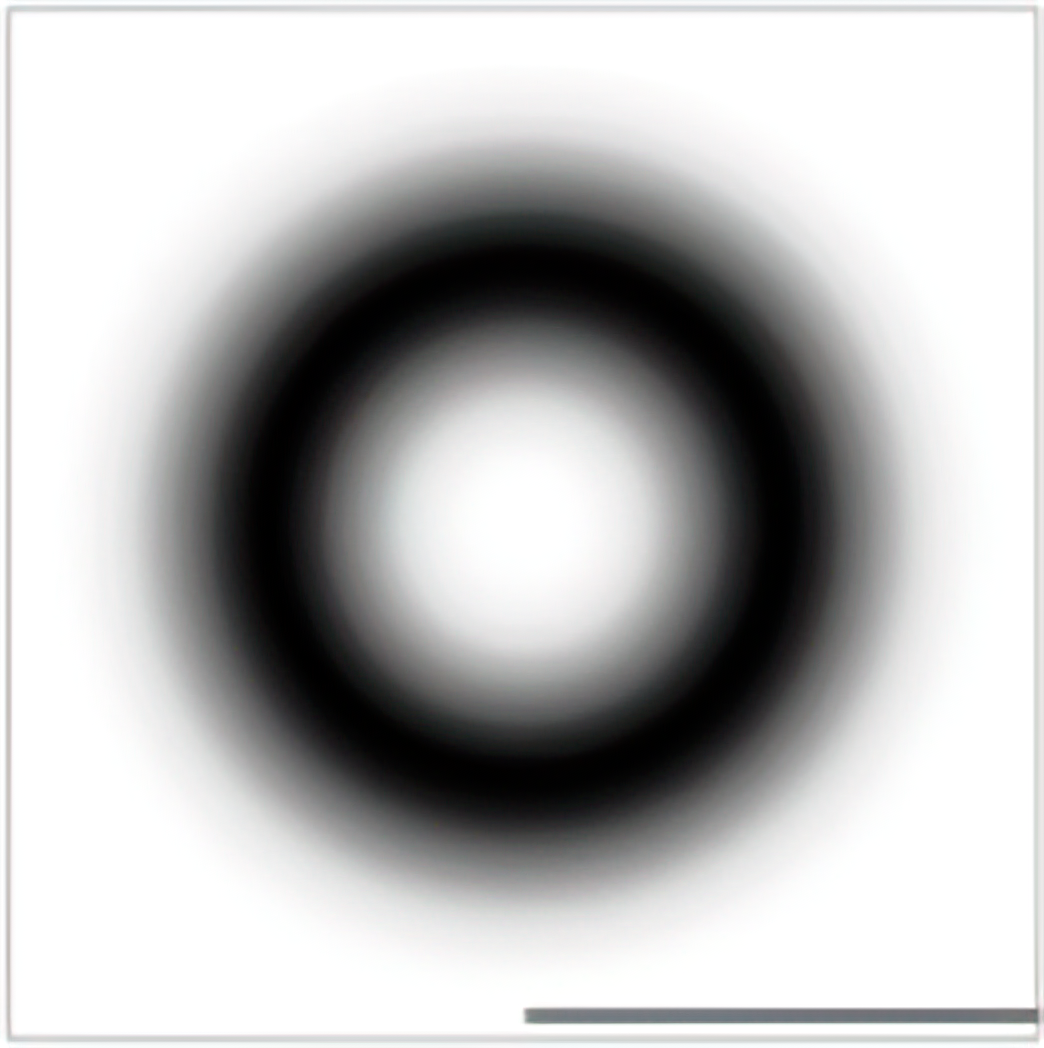
\includegraphics[width=\textwidth]{kernel_shell.png}
        \caption{Kernel-Shell}
        \label{fig:kernels:shell}
    \end{subfigure}
    \hfill
    \begin{subfigure}[t]{0.2\textwidth}
        \centering
        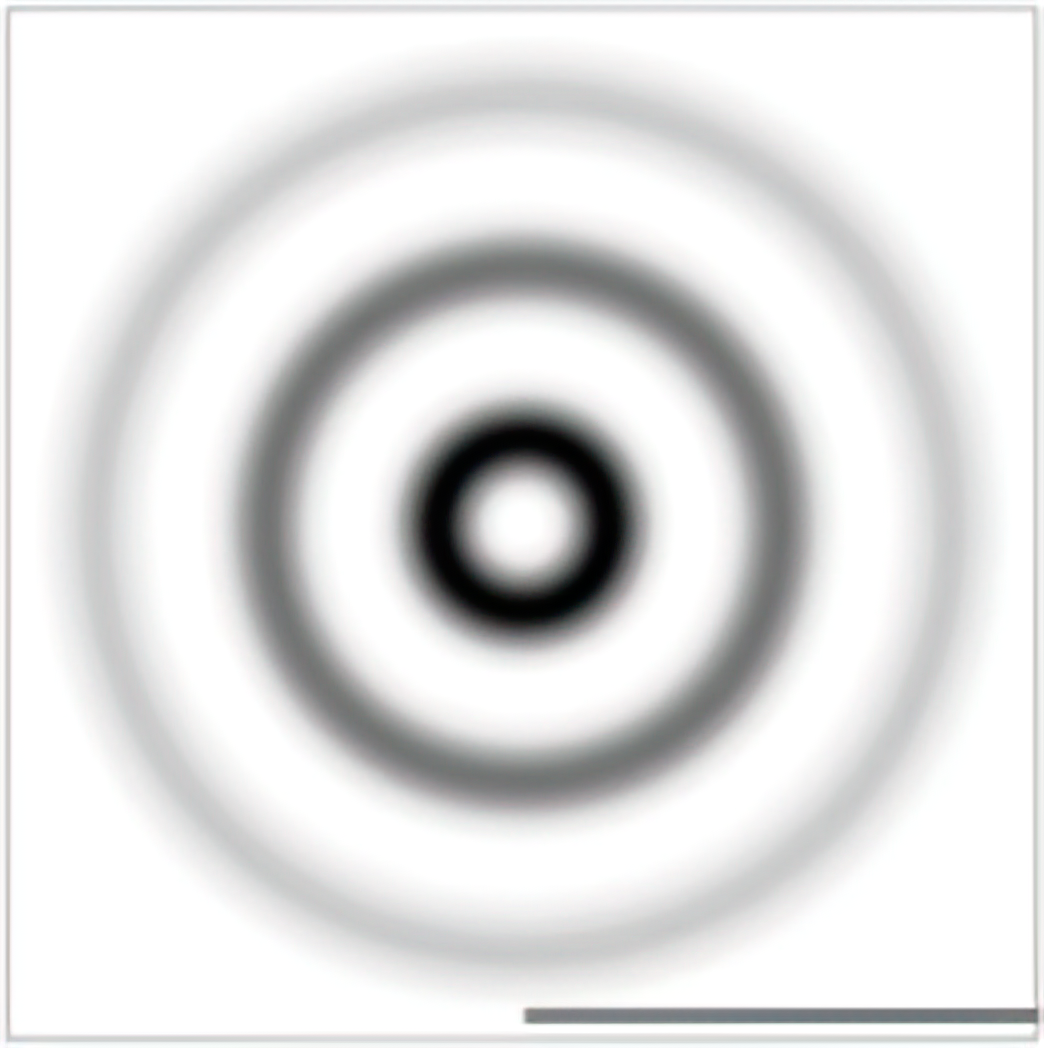
\includegraphics[width=\textwidth]{kernel_skeleton.png}
        \caption{Kernel-Skeleton}
        \label{fig:kernels:skeleton}
    \end{subfigure}
    \caption{\cite{chan2018lenia}}
    \label{fig:kernels}
\end{figure}

\subsection{Lenia}
Der Lenia-Algorithmus gehört ebenfalls zur Familie der zellulären Automaten, unterscheidet sich jedoch von Conway's Game of Life durch sein kontinuierliches System.
Eine Zelle kann nicht nur lebendig oder tot sein, sondern auch einen beliebigen Zustand zwischen 0 und 1 annehmen.
Die Moore-Nachbarschaft wurde durch eine von der Distanz abhängige Nachbarschaft ersetzt, die es ermöglicht, die Nachbarschaft zu erweitern und zu gewichten.
Die Regeln von Conway's Game of Life wurden durch eine Kernel- und eine Growth-Funktion ersetzt, die die Veränderung der Zellen im nächsten Schritt bestimmen.
Zuerst wird mithilfe eines Radius eine Nachbarschaft um die Zelle gebildet.
Die Zustände der Zellen in der Nachbarschaft werden dann mit der Kernel-Funktion gewichtet und anschließend mit der Growth-Funktion zu einem neuen Wert zusammengefasst.
Dieser wird gewichtet auf die Zelle addiert und ergibt den neuen Zustand der Zelle.
Der Kernel besteht aus zwei Teilen: der \textit{Kernel-Shell} und dem \textit{Kernel-Skeleton}.
Für die Kernel-Shell kann beispielsweise die Exponentialfunktion $K_C(r) = \exp\left(\operatorname{4 - \frac{4}{4r(1-r)}}\right)$ gewählt werden, welche wie ~\autoref{fig:kernels:shell} aussieht und die Nachbarschaft gewichtet.
Hierbei ist zu beachten, dass der Radius $r$ auf einem Bereich zwischen 0 und 1 normiert ist.
Soll dies nun auf einem Mesh stattfinden, so bietet es sich an, zuerst die durchschnittliche Kantenlänge der Faces zu bestimmen und ein Vielfaches davon als Norm für den Radius zu wählen.
Des Weiteren lässt sich die Distanz zwischen zwei Faces eines Meshes entweder durch die euklidische Distanz oder durch die Distanz auf der Oberfläche bestimmen.
Die geodätische Distanz ist die kürzeste Distanz zwischen zwei Punkten auf einer Oberfläche.
Es gibt verschiedene Algorithmen zur Bestimmung dieser Distanz, die sich in Genauigkeit und Laufzeit unterscheiden.
Die meisten davon sind jedoch darauf ausgelegt, die Distanz zwischen zwei Vertices und nicht zwischen zwei Faces zu bestimmen.
Wird nun zuerst das duale Mesh bestimmt, so wird das Zentrum eines Faces zu einem Vertex und die Kanten zu Faces.
Die Distanz zwischen zwei Faces ist dann die Distanz zwischen den zugehörigen Vertices.
Alle Faces, die innerhalb des Radius liegen, werden dann in die Nachbarschaft aufgenommen.
Zusätzlich zur Kernel-Shell können noch Peaks hinzugefügt werden, welche in das Kernel-Skeleton einfließen.
Die Peaks sind dabei in einer Liste gespeichert $\beta = \{\beta_0, ..., \beta_{n-1}\} \in [0,1]^n$ und das Kernel-Skeleton ergibt sich wie folgt:
\[
    \operatorname{K_S}(r) = \beta_{\lfloor n \cdot r \rfloor} \cdot \operatorname{K_C}(n \cdot r \bmod 1)
\]
$n$ gibt dabei die Anzahl der Peaks an, $r$ ist die zwischen 0 und 1 normierte Distanz und $\bmod 1$ gibt den Nachkommateil von $n \cdot r$ an.
Die für $\beta$ verwendeten Werte geben dabei die Gewichtung der Peaks an. ~\autoref{fig:kernels:skeleton} zeigt ein Beispiel für ein Kernel-Skeleton mit drei verschiedenen Peaks.
Damit der Kernel vollständig ist, muss dieser nun noch normiert werden. Dies geschieht für eine Zelle wie folgt:
\[
    \begin{aligned}
        N                      & := \text{Menge aller Nachbarn der betrachteten Zelle}                                                                                                     \\
        n                      & := \text{ein Nachbar der betrachteten Zelle}                                                                                                              \\
        \operatorname{dist}(n) & := \text {Distanz zwischen betrachteter Zelle und Zelle n}                                                                                                \\
        \operatorname{area}(n) & := \text {Fläche von Zelle n}                                                                                                                             \\
        \operatorname{K}(n)    & := \frac{\operatorname{K_S}(\operatorname{dist}(n))}{\sum_{n \in N} \left(\operatorname{K_S}(\operatorname{dist}(n)) \cdot \operatorname{area}(n)\right)}
    \end{aligned}
\]
Der Nenner sorgt dabei für die Normierung des Kernels, was durch die noch folgenden Gleichungen deutlich wird.
Ist nun der Kernel vollständig, so lässt sich ein Zwischenwert für die Zelle in Abhängigkeit von der Nachbarschaft bestimmen:
\[
    \begin{aligned}
        x                     & := \text{betrachtete Zelle}                                                                                \\
        \operatorname{A}^t(x) & := \text{aktueller Zustand der Zelle x}                                                                    \\
        \operatorname{U}(x)   & = \sum_{n \in N} \left(\operatorname{K}(n) \cdot \operatorname{A}^t(n) \cdot \operatorname{area}(n)\right)
    \end{aligned}
\]
Nachdem der Zwischenwert für die Zelle bestimmt wurde, wird dieser durch die Growth-Funktion zu einem neuen Wert zusammengefasst.
Die Growth-Funktion ist eine beliebige, kontinuierliche Funktion, die den Zwischenwert, welcher zwischen 0 und 1 liegt, auf einen neuen Wert zwischen -1 und 1 abbildet.
Hier kann beispielsweise eine Exponentialfunktion $\operatorname{G}(u) = 2 \cdot \exp \left(-\frac{(u - \mu)^2}{2 \cdot \sigma^2}\right) - 1$ gewählt werden.
Die Parameter $\mu$ und $\sigma$ können dabei frei angepasst werden.
$\mu$ gibt das Maximum und $\sigma$ die Breite der Funktion an.
~\autoref{fig:expgrowth} zeigt ein Beispiel für verschiedene Parameter.
Ist $\sigma$ ein kleiner Wert, so werden mehr Werte auf -1 abgebildet, wodurch die Zellen schneller sterben.
Nachdem die Growth-Funktion bestimmt wurde, folgt die Aktualisierung der Zelle.
Dafür wird der neue Wert der Zelle mit einem Gewicht auf den alten Wert addiert und zwischen 0 und 1 begrenzt.
\[
    \begin{aligned}
        \operatorname{A}^{t+1}(x)  & := \text{neuer Zustand der Zelle x}                                                                                           \\
        g                          & := \text{Gewichtungsfaktor}                                                                                                   \\
        \operatorname{clip}(u,v,w) & := \operatorname{max}(u, \operatorname{min}(v, w))                                                                            \\
        \operatorname{A}^{t+1}(x)  & := \operatorname{clip}\left(\operatorname{A}^{t+1}(x) + g \cdot \operatorname{G}\left(\operatorname{U}(x)\right), 0, 1\right)
    \end{aligned}
\]
Damit ist die Aktualisierung einer Zelle für einen Zeitschritt abgeschlossen.
Der Gewichtungsfaktor $g \in (0,1]$ und der Zeitschritt $t+1$ bestimmen dabei die zeitliche Auflösung des Systems.
Je kleiner der Gewichtungsfaktor, desto langsamer und flüssiger entwickelt sich das System.

\begin{figure}[!htbp]\centering
    \begin{subfigure}[t]{0.2\textwidth}
        \centering
        \begin{tikzpicture}
            \begin{axis}[
                    axis lines=middle,
                    xmin=0, xmax=1,
                    ymin=-1, ymax=1,
                    xlabel=$u$,
                    ylabel=$\operatorname{G}(u)$,
                    ylabel style={anchor=west},
                    xtick={0,1},
                    ytick={-1,0,1},
                    xticklabels={0,1},
                    yticklabels={-1,0,1},
                    samples=300,
                    width=\textwidth,
                    height=\textwidth,
                ]
                \addplot[domain=-1:1, color=red]{2 * exp(-((x - 0.6)^2)/(2 * 0.1^2)) - 1};
            \end{axis}
        \end{tikzpicture}
        \caption{$\mu = 0.6, \sigma = 0.1$}
        \label{fig:expgrowth:1}
    \end{subfigure}
    \hfill
    \begin{subfigure}[t]{0.2\textwidth}
        \centering
        \begin{tikzpicture}
            \begin{axis}[
                    axis lines=middle,
                    xmin=0, xmax=1,
                    ymin=-1, ymax=1,
                    xlabel=$u$,
                    ylabel=$\operatorname{G}(u)$,
                    ylabel style={at={(1,1)},anchor=east},
                    xtick={0,1},
                    ytick={-1,0,1},
                    xticklabels={0,1},
                    yticklabels={-1,0,1},
                    samples=500,
                    width=\textwidth,
                    height=\textwidth,
                ]
                \addplot[domain=-1:1, color=red]{2 * exp(-((x - 0.15)^2)/(2 * 0.017^2)) - 1};
            \end{axis}
        \end{tikzpicture}
        \caption{$\mu = 0.15, \sigma = 0.017$}
        \label{fig:expgrowth:2}
    \end{subfigure}
    \hfill
    \caption{Exponentialfunktion als Growth-Funktion mit verschiedenen Parametern}
    \label{fig:expgrowth}
\end{figure}

\subsection{Implementierung von Lenia}
Ausgehend davon, dass der Lenia-Algorithmus auf einem statischen Mesh ausgeführt wird, können einige Dinge vorberechnet werden.
Eine naive Implementierung würde für jeden Zeitschritt jede Zelle durchgehen, die Nachbarschaft bestimmen und die benötigten Werte berechnen.
Wenn sich das Mesh und die für den Algorithmus verwendeten Parameter nicht ändern, kann die Nachbarschaft für jede Zelle einmal beim Laden des Meshes bestimmt und danach wiederverwendet werden.
Ebenfalls fällt auf, dass der Wert des Kernels $\operatorname{K}(n)$ von der Distanz zwischen der betrachteten Zelle und der Zelle $n$ abhängt.
Wenn sich die Nachbarschaft einer Zelle nicht ändert, kann der Wert des Kernels für alle Nachbarn einer Zelle einmal berechnet und anschließend wiederverwendet werden.
Hierbei ist zu beachten, dass eine Zelle nicht nur einen Kernel-Wert hat.
Der Kernel-Wert hängt von der Nachbarschaftsrelation ab, weshalb es sinnvoll ist, ihn mit der zuvor erwähnten Nachbarschaftsrelation zu speichern.
Darüber hinaus bleibt die Fläche $\operatorname{area}(n)$ einer Zelle auf einem statischen Mesh konstant, so dass sie ebenfalls vorberechnet werden kann.
Die Kernel-Funktion $\operatorname{K_S}$ und die Funktion $\operatorname{U}$ enthalten beide eine Summe mit derselben Laufvariable und demselben Endwert, sodass sie in der Implementierung in einer Schleife zusammengefasst werden können.
Wenn all diese Werte vorberechnet werden, muss bei der Aktualisierung des Zustands einer Zelle nur der aktuelle Zustand abgefragt und mit bereits berechneten Werten multipliziert werden, um den Kernel-Wert zu erhalten.
Dieser wird dann in die Growth-Funktion eingesetzt und der neue Zustand der Zelle bestimmt.
Bei der Aktualisierung des Zustands des gesamten Systems wird jede Zelle durchlaufen und anhand der zuvor bestimmten Nachbarschaft der neue Zustand bestimmt.
Da der nächste Zustand immer nur vom aktuellen Zustand abhängt, kann dieser Prozess parallelisiert werden.
Der Wert jeder Zelle kann unabhängig von den anderen Zellen bestimmt werden.
Dadurch lässt sich die Berechnung des nächsten Zustands auf mehrere Threads aufteilen und beschleunigen.
\section{Ray-Marching}
Eine weitere Möglichkeit, biologisch inspirierte Strukturen zu erzeugen, sind Fraktale.
Fraktale sind selbstähnliche Strukturen, die immer feiner aufgelöst werden können.
Es ist möglich, diese Fraktale als Meshes zu modellieren und auf herkömmliche Weise zu rendern.
Allerdings ist dies nur bis zu einem gewissen Punkt praktikabel.
Ein alternatives Verfahren zum Rendern der Strukturen ist das Ray-Marching, bei welchem die Strukturen nicht als Meshes, sondern als implizite Funktionen dargestellt werden \cite{wikipedia_raymarching}.

\begin{figure}[!htbp]\centering
    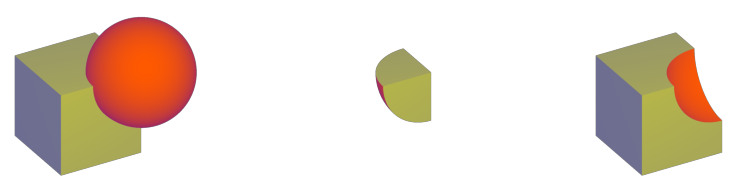
\includegraphics[width=0.4\textwidth]{csg_operations.png}
    \caption{\cite{fotonixx_csg}}
    \label{fig:bool_ops}
\end{figure}

\subsection{Darstellung von Objekten} \label{sec:ray_marching:objects}
Die Darstellung von Objekten erfolgt mittels \emph{Signed Distance Functions} (SDF).
Diese Funktionen geben für einen bestimmten Punkt im Raum den Abstand zur Oberfläche eines Objekts an.
Die Funktionen können sowohl positive als auch negative Werte zurückgeben, je nachdem, ob sich der Punkt innerhalb oder außerhalb der Struktur befindet.
Ein Beispiel für eine primitive Funktion ist die einer Kugel im Ursprung mit einem Radius von 1.
Diese kann als $||p||_2 - r$ beschrieben werden, wobei $||p||_2$ der euklidische Abstand des Punktes $p$ zum Ursprung und $r$ der Radius der Kugel ist.
Wenn $p$ innerhalb der Kugel liegt, ist der Abstand negativ, wenn $p$ außerhalb der Kugel liegt, ist der Abstand positiv und wenn $p$ genau auf der Oberfläche der Kugel liegt, ist der Abstand 0.
Für eine Vielzahl von primitiven und komplexeren Strukturen können solche SDFs gefunden werden \cite{iquilezles_distfunctions}.
Befinden sich nun zwei oder mehr Objekte im Raum, so können diese durch verschiedene Operationen miteinander verknüpft werden.
Wenn das Minimum der beiden Funktionen gebildet wird, ergibt sich eine neue Funktion, die den Abstand zum nächstgelegenen der beiden Objekte angibt.
Beim Maximum der beiden Funktionen, ergibt sich eine Funktion, die den Schnitt der beiden Objekte beschreibt.
Es ist auch möglich, ein Objekt von dem anderen zu subtrahieren, indem das Maximum eines Objekts zusammen mit dem negativen Wert des anderen Objekts, das von dem ersten Objekt abgezogen werden soll, gebildet wird.
\autoref{fig:bool_ops} zeigt die Vereinigung und den Schnitt eines Würfels mit einer Kugel sowie das Ergebnis, wenn die Kugel von dem Würfel subtrahiert wird.


\subsection{Ray-Marching-Algorithmus}
Zum Darstellen der Objekte wird ein Ray-Marching-Algorithmus verwendet.
Dabei wird für jedes Pixel des Bildes ein Strahl von der Kamera in die Szene geschickt.
Mit Hilfe der SDF kann der Abstand zum nächsten Objekt bestimmt werden.
Obwohl nicht bekannt ist, wo sich das nächstgelegene Objekt befindet, kann sichergestellt werden, dass der Strahl nicht zu weit in die Szene hineingeschickt wird.
Der Strahl läuft dann um den berechneten Abstand weiter in die vorgegebene Richtung und von diesem Punkt aus wird erneut der Abstand zum nächsten Objekt berechnet.
Dieser Vorgang wird iterativ wiederholt, bis entweder ein oberes Limit an Iterationen erreicht ist, eine maximal zulässige Distanz überschritten wurde oder der Abstand zum nächsten Objekt kleiner als ein vorgegebenes Minimum ist.
Wenn dieses Minimum erreicht ist, wird angenommen, dass der Strahl auf ein Objekt trifft.
Wenn das obere Limit der Iterationen erhöht oder das Minimum verringert wird, erhöht sich die Genauigkeit des Algorithmus, wodurch die Objekte höher aufgelöst werden, aber auch die Laufzeit steigt.

\begin{figure}[!htbp]\centering
    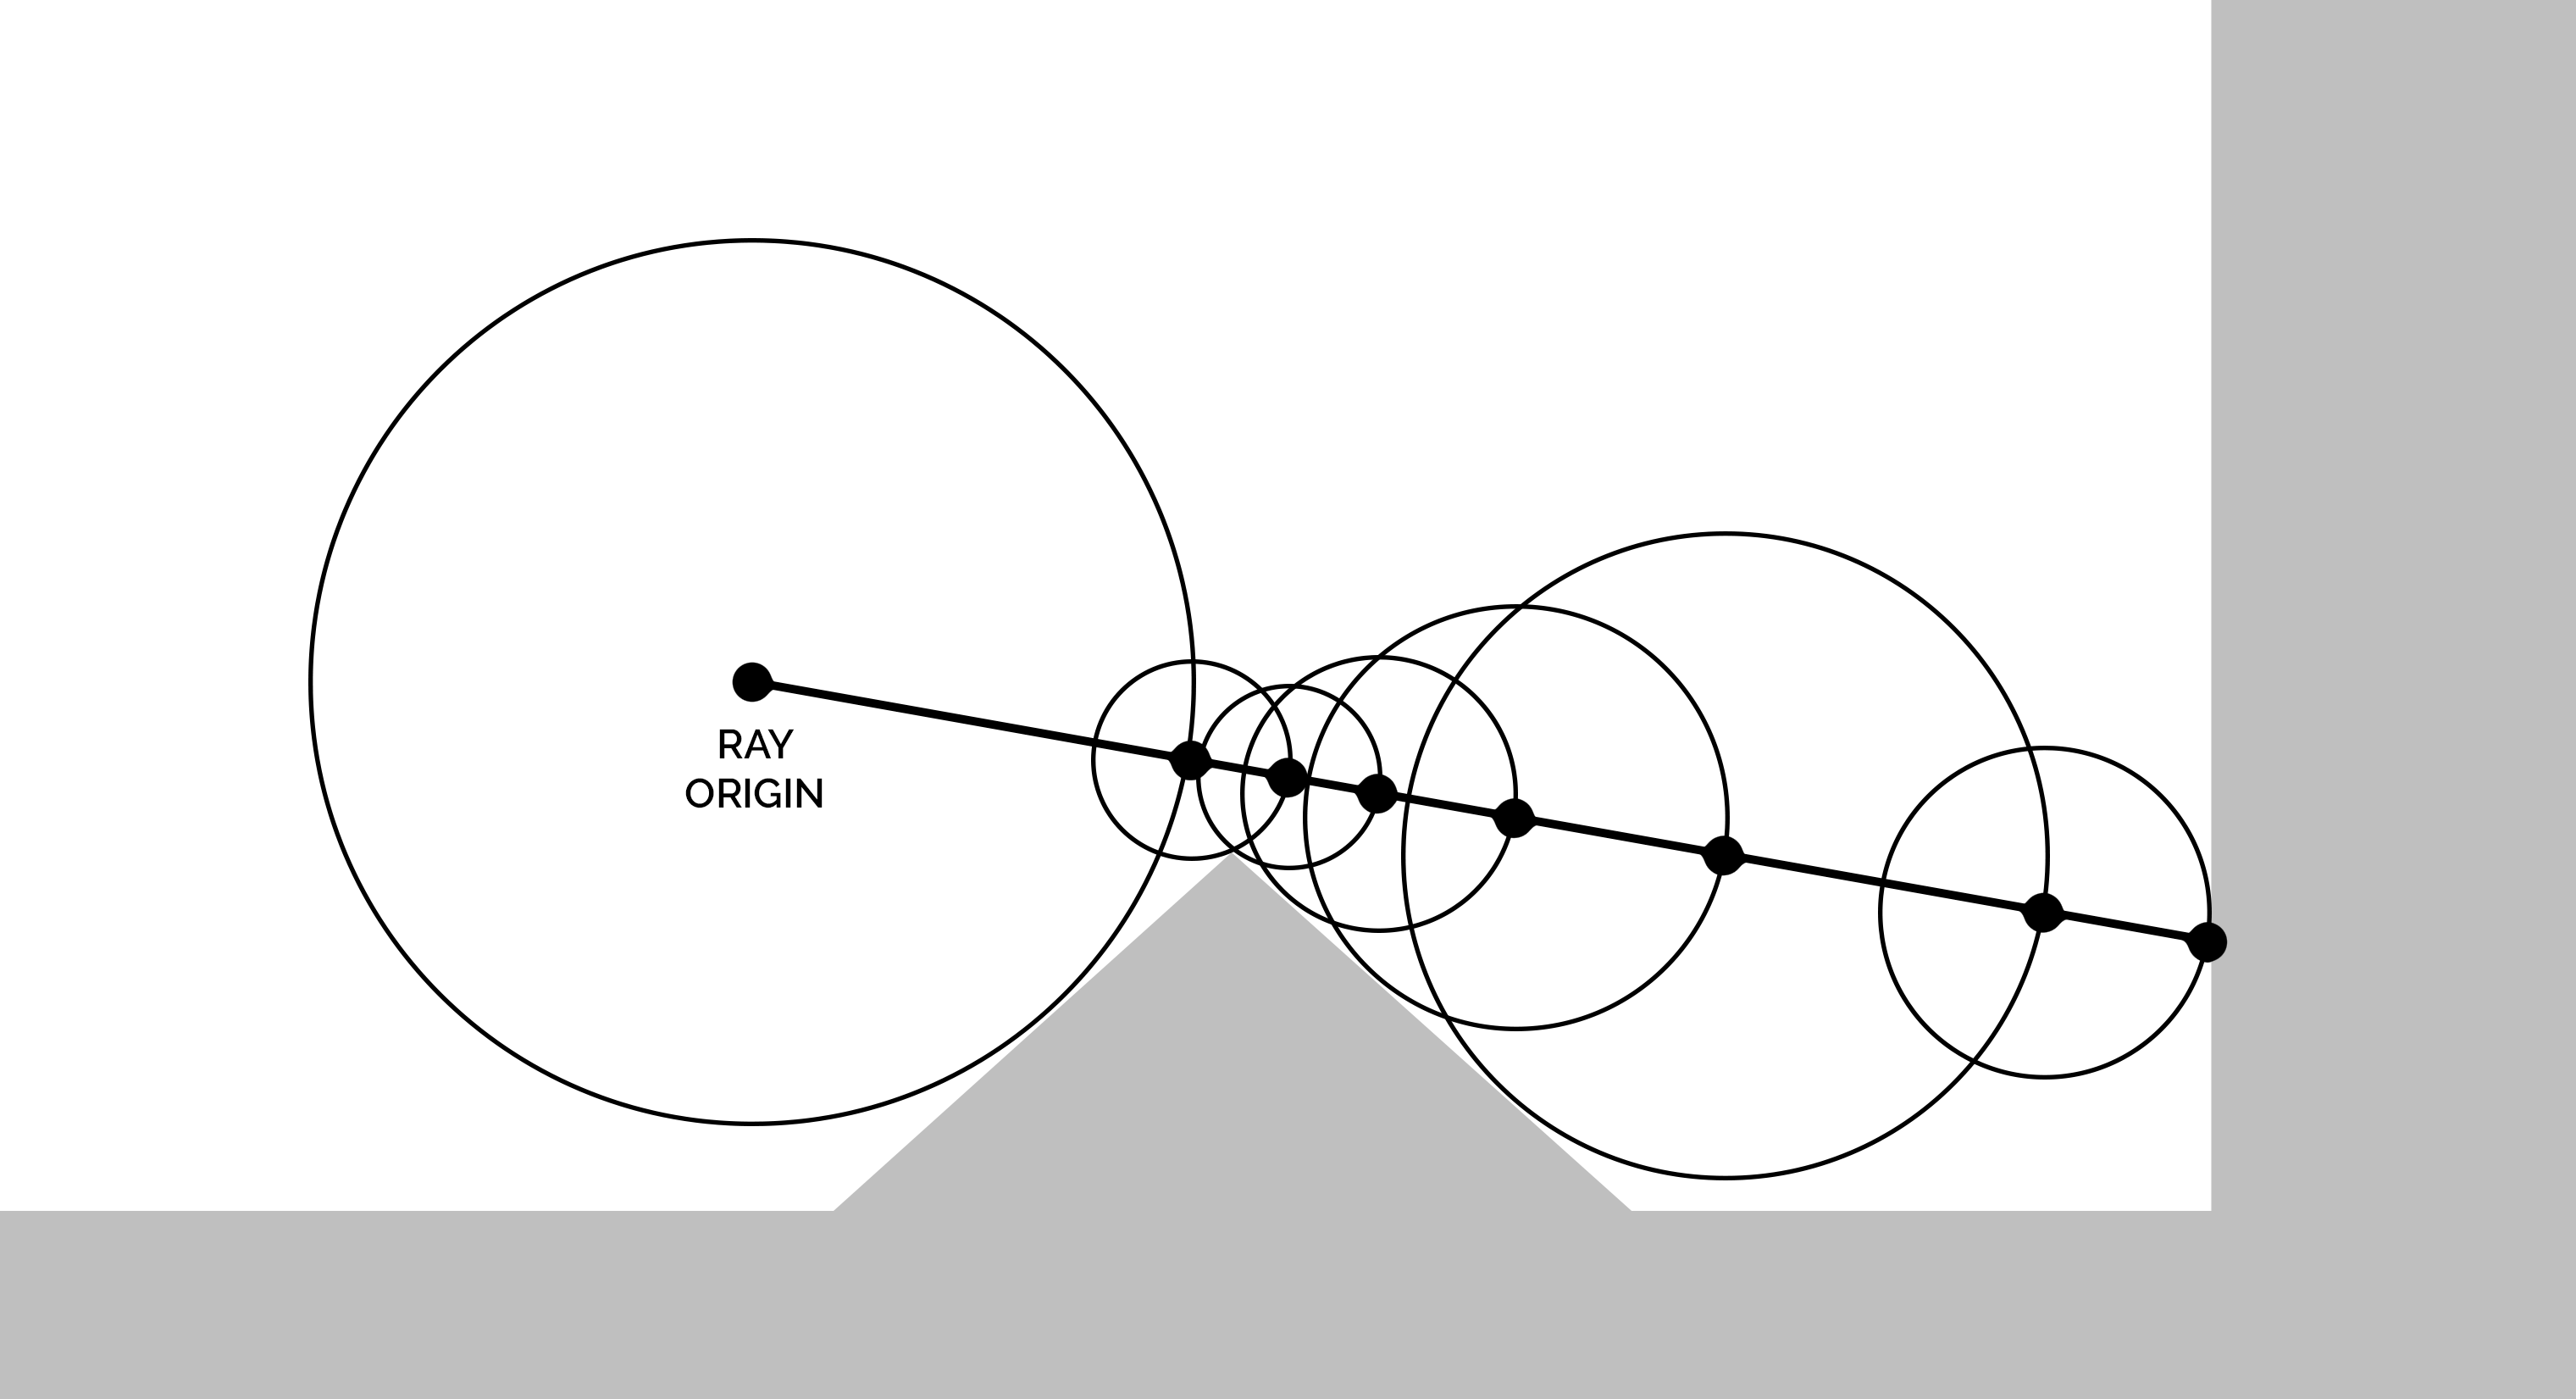
\includegraphics[width=0.5\textwidth - 7.82454pt]{Visualization_of_SDF_ray_marching_algorithm.png}
    \caption{Visualisierung des Ray-Marching-Algorithmus. \cite{wikimedia_sdf}}
    \label{fig:ray_marching}
\end{figure}

\begin{figure}[!htbp]\centering
    \begin{subfigure}[t]{0.2\textwidth}
        
\includegraphics[width=\textwidth]{Viewer0.png}
        \caption{Keine Beleuchtung}
        \label{fig:lighting:none}
    \end{subfigure}
    \hfill
    \begin{subfigure}[t]{0.2\textwidth}
        \centering
        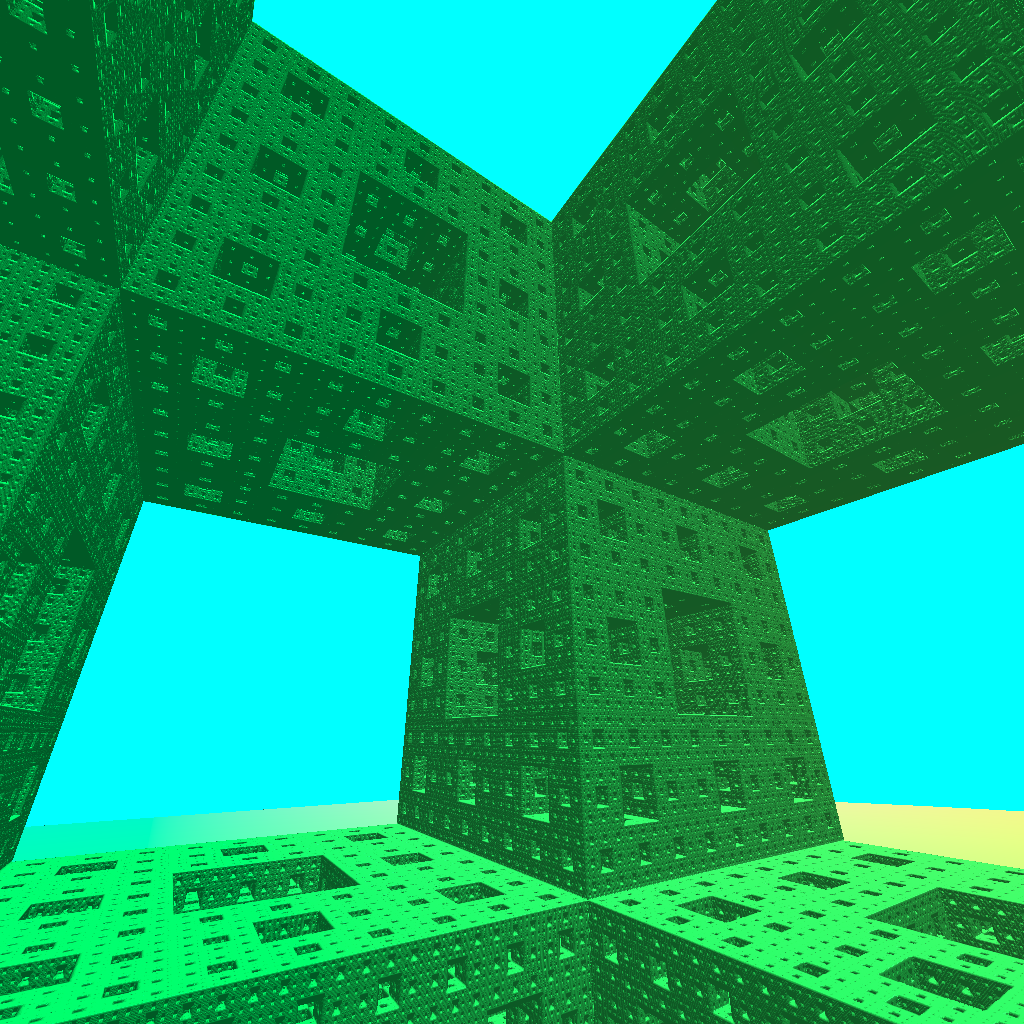
\includegraphics[width=\textwidth]{Viewer1.png}
        \caption{Phong-Beleuchtung}
        \label{fig:lighting:phong}
    \end{subfigure}
    \hfill
    \begin{subfigure}[t]{0.2\textwidth}
        \centering
        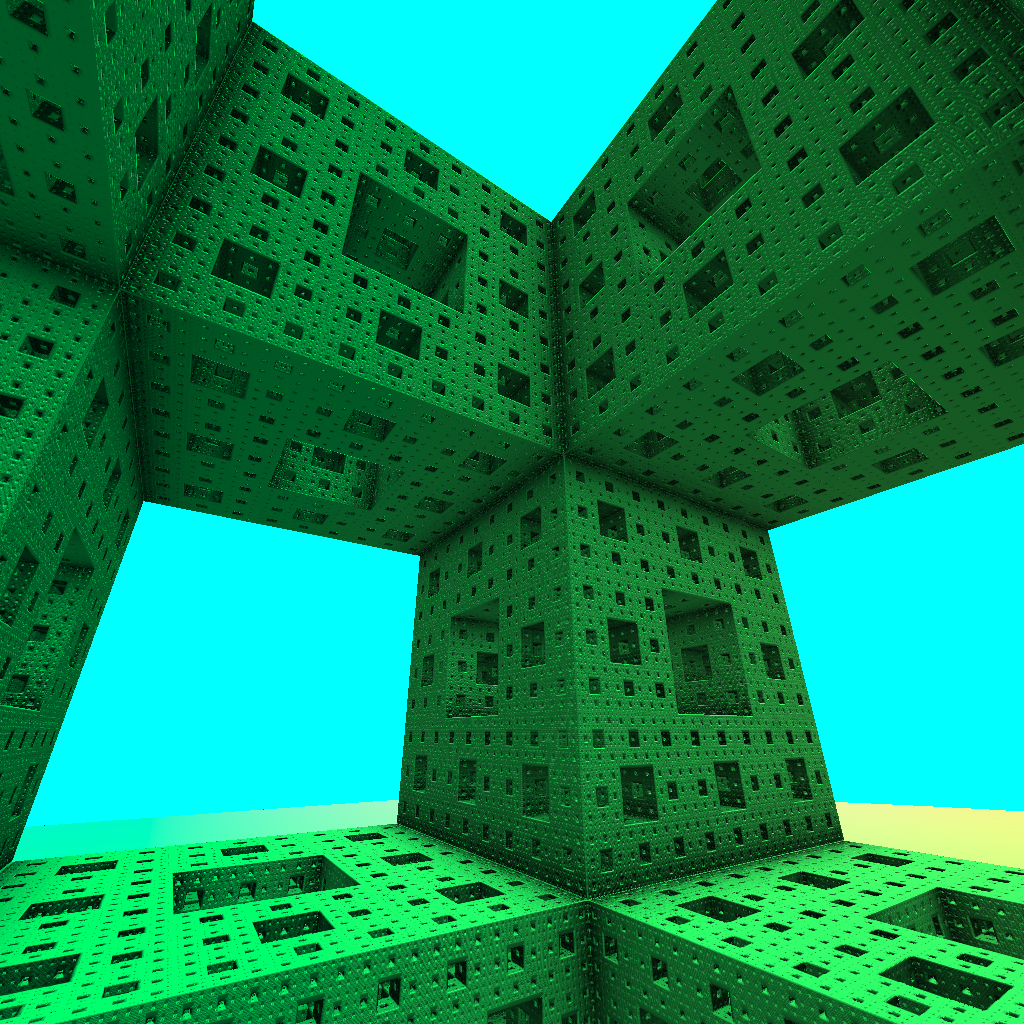
\includegraphics[width=\textwidth]{Viewer2.png}
        \caption{Ambient Occlusion}
        \label{fig:lighting:ao}
    \end{subfigure}
    \hfill
    \begin{subfigure}[t]{0.2\textwidth}
        \centering
        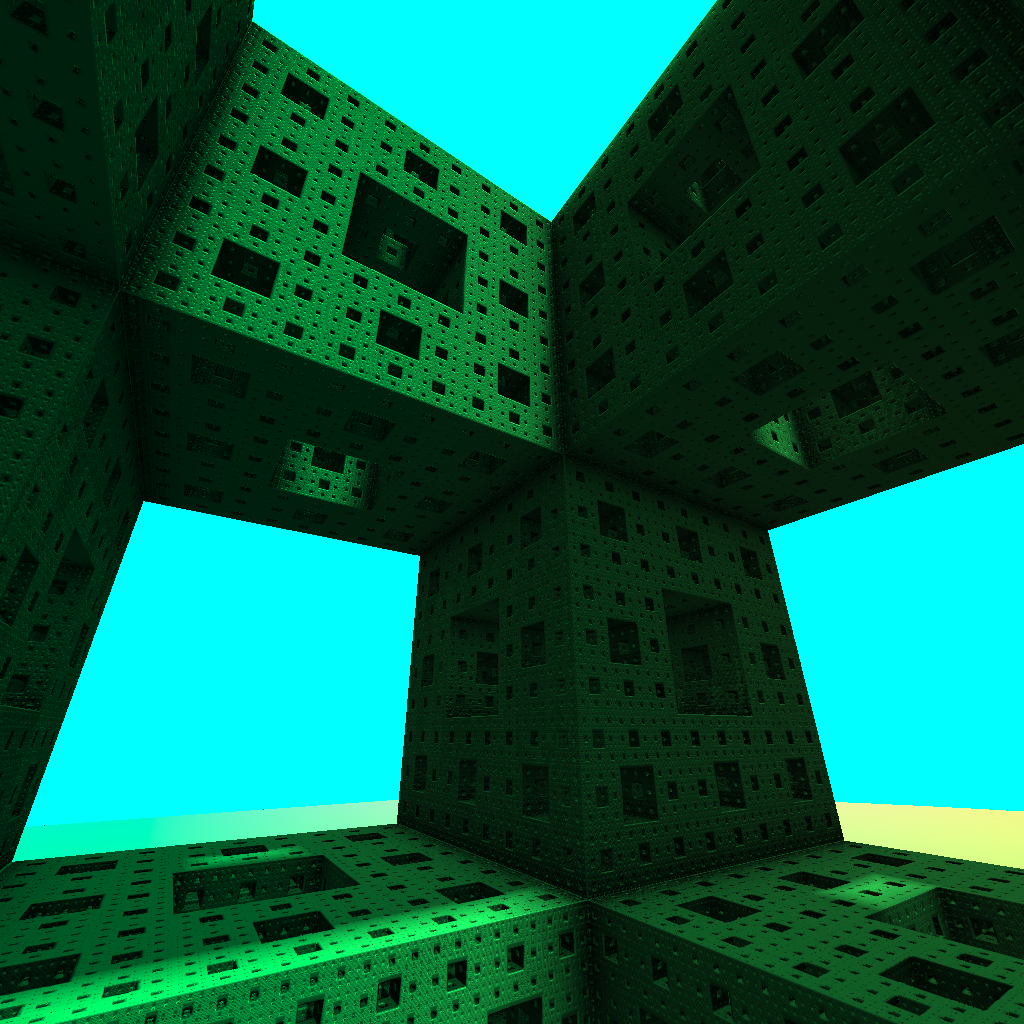
\includegraphics[width=\textwidth]{Viewer3.png}
        \caption{Soft Shadows}
        \label{fig:lighting:soft}
    \end{subfigure}
    \caption{Inkrementelles Hinzufügen von Beleuchtungseffekten}
    \label{fig:lighting}
\end{figure}

\subsection{Licht und Schatten}
Trifft nun ein Strahl auf ein Objekt, so kann für diesen Punkt ein Beleuchtungsmodell ausgewertet werden.
Wird dafür beispielsweise das Phong-Beleuchtungsmodell verwendet, so wird dafür die Normale an dem Punkt benötigt.
Für einfache Objekte wie Kugeln oder Flächen kann diese Normale unkompliziert bestimmt werden, für komplexere Strukturen kann dies jedoch schwierig sein.
Die Normale eines Punktes kann mit dem Gradienten der SDF an diesem Punkt bestimmt werden.
Dies kann numerisch approximiert werden, indem die SDF um den Punkt herum in alle drei Richtungen mit einem kleinen Abstand ermittelt und der Abstand zum Punkt berechnet wird.
Dies entspricht der Bestimmung des Gradienten der SDF an diesem Punkt, womit die Normale an diesem Punkt bestimmt werden kann.
Ist die Normale an dem Punkt bekannt, so kann das bekannte Phong-Beleuchtungsmodell verwendet werden, um die Beleuchtung an dem Punkt auszuwerten, wie in \autoref{fig:lighting:phong} zu sehen ist.

Mithilfe der Normalen lässt sich ebenfalls Ambient Occlusion bestimmen.
Dazu wird von einem Oberflächenpunkt aus entlang der Richtung der Normale ein Strahl in die Szene geschickt und dabei der Abstand zum nächsten Objekt bestimmt.
Dies geschieht für eine feste Anzahl von Schritten, wobei in jedem Schritt die Weite des Strahls vergrößert wird.
Dabei werden die ermittelten Entfernungen und die vom Strahl zurückgelegte Distanz aufsummiert.
Wenn kein anderes Objekt in der Nähe liegt, ist die Summe der Objektentfernungen $S$ gleich der Summe der zurückgelegten Distanzen $M$, da die SDF in jedem Schritt den Abstand zum Ausgangspunkt zurückgeben würde.
Wenn ein anderes Objekt in der Nähe ist, wäre $S$ kleiner als $M$.
$S \div M$ ergibt dann einen Wert zwischen 0 und 1, der als Ambient Occlusion-Wert verwendet werden kann, indem er mit dem Farbwert des Punktes multipliziert wird.
Dieses Verfahren kann verfeinert werden, indem weiter entfernte Distanzen weniger stark gewichtet werden \cite{zucconi_ao}.
Das Ergebnis ist in \autoref{fig:lighting:ao} dargestellt.

Eine einfache Möglichkeit Schatten zu erzeugen besteht darin, von jedem Punkt auf der Oberfläche einen Strahl zur Lichtquelle zu senden und zu überprüfen, ob dieser Strahl auf ein Objekt trifft.
Wenn der Strahl auf ein Objekt trifft, liegt der Punkt im Schatten und es wird ein dunklerer Farbwert verwendet.
Dieses Verfahren erzeugt scharfe Schatten, die jedoch nicht immer erwünscht sind.
Wenn ein Strahl auf dem Weg zwischen dem Punkt und der Lichtquelle ein Objekt nur knapp verfehlt, könnte dieser im Halbschatten liegen, um ein weicheres Schattenbild zu erzeugen.
Für jeden Schritt der Ray-Marching-Iteration zwischen Punkt und Lichtquelle kann ein Halbschatten-Faktor bestimmt werden.
Dieser ergibt sich aus dem Wert der SDF des aktuellen Punktes der Iteration, der ins Verhältnis zur Distanz zum Ausgangspunkt gesetzt wird, sodass weiter entfernte Objekte weniger stark gewichtet werden.
Von den bestimmten Halbschatten-Faktoren entlang des Strahls wird dann der kleinste Wert verwendet, um den Farbwert des Punktes zu bestimmen.
Aufgrund der geringeren Gewichtung der Werte für weiter entfernte Objekte entsteht außerdem der Effekt, dass die Schatten weicher werden, je weiter sie von dem Objekt entfernt sind und umgekehrt \cite{iquilezles_rmshadows}.
Dieser Effekt ist in \autoref{fig:shadows:soft} dargestellt.

\begin{figure}[!htbp]\centering
    \begin{subfigure}[t]{0.2\textwidth}
        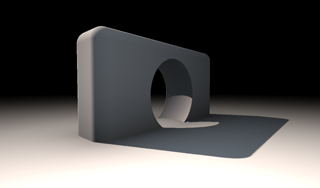
\includegraphics[width=\textwidth]{gfx12.png}
        \caption{Hard Shadow}
        \label{fig:shadows:hard}
    \end{subfigure}
    \hfill
    \begin{subfigure}[t]{0.2\textwidth}
        \centering
        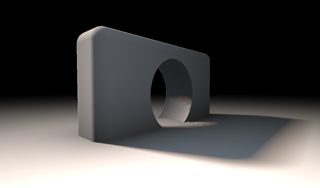
\includegraphics[width=\textwidth]{gfx08.png}
        \caption{Soft Shadow}
        \label{fig:shadows:soft}
    \end{subfigure}
    \caption{\cite{iquilezles_rmshadows}}
    \label{fig:shadows}
\end{figure}


\subsection{Fraktalstrukturen}
Um fraktalartige Strukturen zu erstellen, können SDFs verwendet werden, die sich unendlich oft wiederholen.
Eine Kugel, die mit einer SDF dargestellt wird und deren untere linke Ecke im Ursprung liegt und einen Radius von 1 hat, ist in \autoref{fig:sphere:simple} dargestellt.
Die SDF nimmt einen Punkt im Raum als Eingabe und gibt den Abstand zu der Oberfläche der Kugel zurück.
Dieser Punkt im Raum ist der aktuelle Punkt der Ray-Marching-Iteration.
Wenn auf die x-, y- und z-Koordinate dieses Punktes der Modulo-Operator mit beispielsweise 5 angewendet wird, liegen die jeweiligen Werte immer zwischen 0 und 5.
Das bedeutet, dass wenn der Strahl auf der x-Achse nach rechts die 5 überschreiten würde, er dies nicht tut und stattdessen von links wieder bei 0 anfängt.
Geschieht dies für alle Achsen, ergibt sich ein impliziter Kasten mit einer Kantenlänge von 5.
Alle Objekte innerhalb dieses Kastens werden aufgrund der Modulo-Operation unendlich oft in alle Richtungen wiederholt.
\autoref{fig:sphere:inf} zeigt, wie dies für eine Kugel aussehen kann.
Wenn dies nur in einer Achsenrichtung geschehen soll, kann der Modulo-Operator nur auf eine Achse angewendet werden.

\begin{figure}[!htbp]\centering
    \begin{subfigure}[t]{0.2\textwidth}
        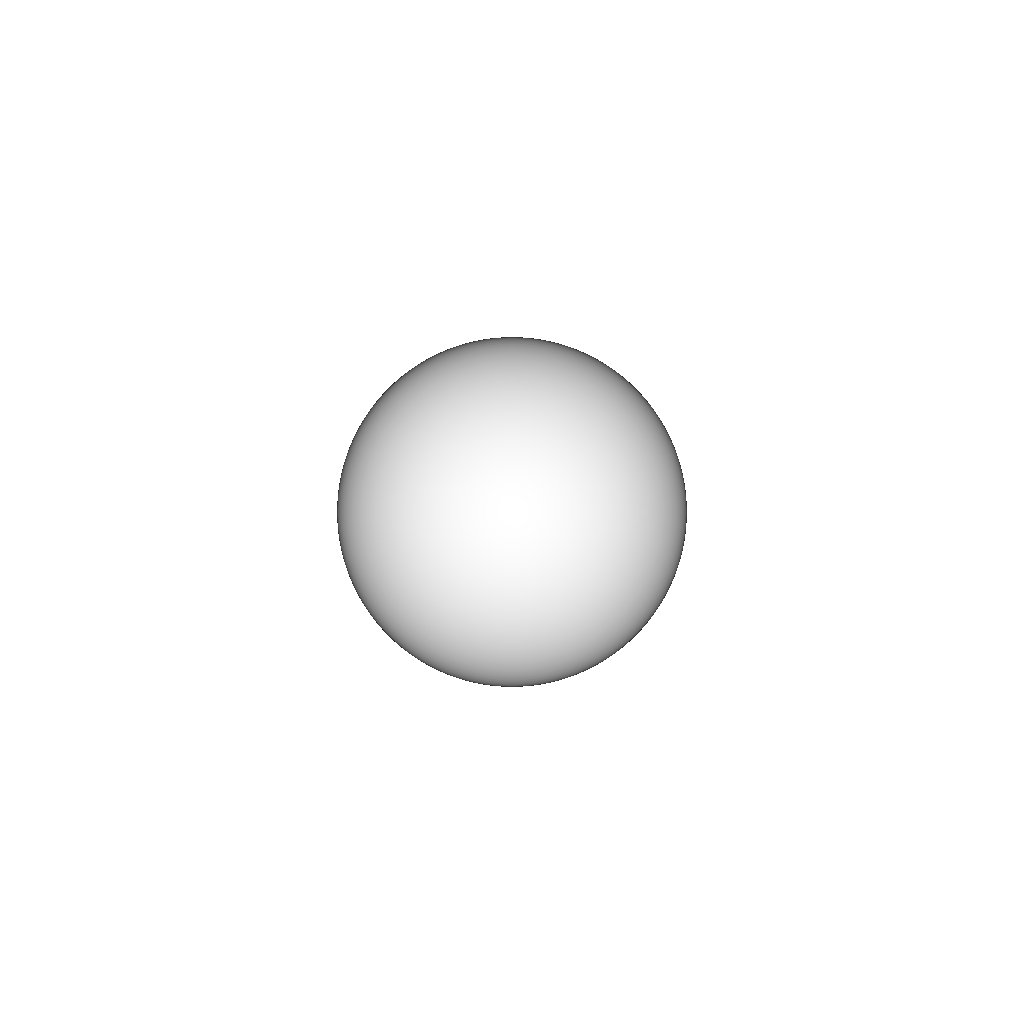
\includegraphics[width=\textwidth]{sphere0.png}
        \caption{}
        \label{fig:sphere:simple}
    \end{subfigure}
    \hfill
    \begin{subfigure}[t]{0.2\textwidth}
        \centering
        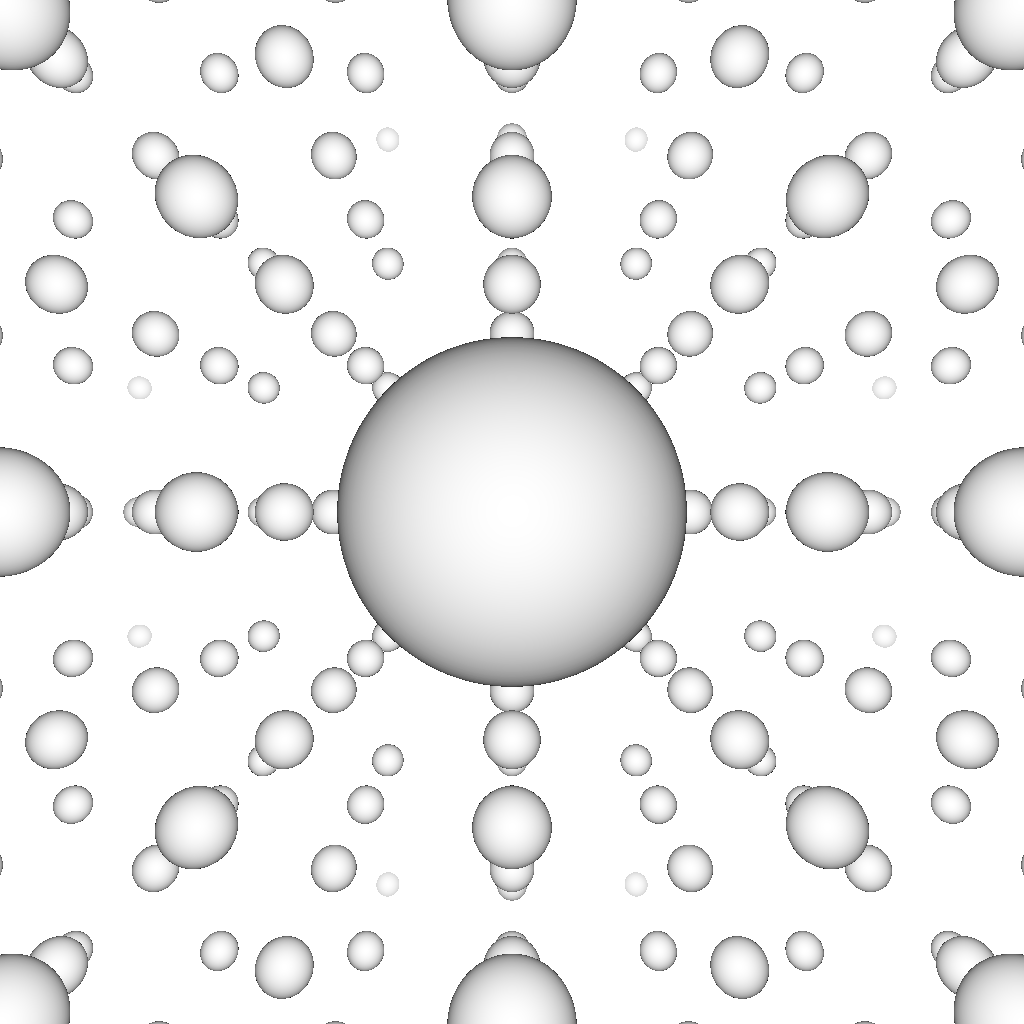
\includegraphics[width=\textwidth]{sphere1.png}
        \caption{}
        \label{fig:sphere:inf}
    \end{subfigure}
    \caption{}
    \label{fig:sphere}
\end{figure}


Der \textit{Menger-Sponge} ist ein Beispiel für eine fraktale Struktur, die sich mit den vorgestellten Methoden dargestellt lässt.
Dazu wird zunächst mit einem Würfel begonnen.
Von diesem wird dann ein Kreuz, wie in \autoref{fig:menger:cross0} zu sehen, mithilfe der in Kapitel \ref{sec:ray_marching:objects} beschriebenen Operationen abgezogen.
Anschließend wird das Kreuz auf $1/3$ seiner vorherigen Größe skaliert und mit dem zuvor erklärten Verfahren in alle Richtungen unendlich oft wiederholt und ebenfalls von dem Würfel abgezogen.
Dieses Verfahren wird nun iterativ wiederholt, bis der Menger-Sponge die gewünschte Auflösung erreicht hat.
\autoref{fig:menger} zeigt dieses iterative Verfahren.
Dabei ist in grün die aktuelle Iteration zu sehen und in rot die Kreuze, die abgezogen werden, um in den nächsten Iterationsschritt zu gelangen.
Zur Veranschaulichung sind diese auf den Bereich des Würfels beschränkt.
Der dadurch entstehende Menger-Sponge ist auch wieder eine SDF, da das beschriebene Verfahren nur das Maximum von zwei SDFs bildet und somit selbst auch wieder eine SDF ist.
Es wäre daher beispielsweise möglich, unendlich viele Menger-Sponges nebeneinander zu platzieren oder einen solchen von anderen Objekten abzuziehen, beziehungsweise andere Objekte von diesem abzuziehen, um so komplexere Strukturen zu erzeugen.
Da eine Signed Distance Function nicht nur als mathematische Funktion, sondern auch als eine aus Programmiersprachen bekannte Funktion verstanden werden kann, lassen sich damit viele weitere interessante Strukturen erzeugen.

\begin{figure}[!htbp]\centering
    \begin{subfigure}[t]{0.11\textwidth}
        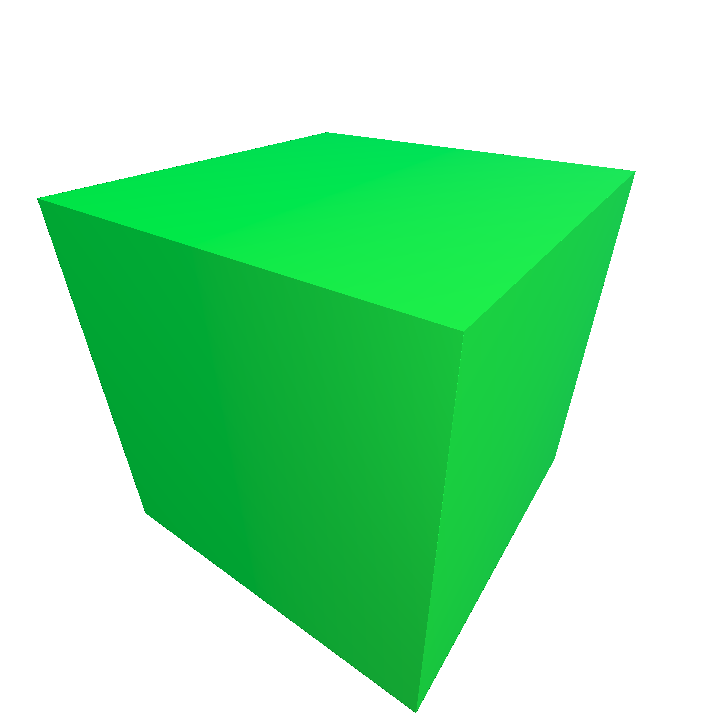
\includegraphics[width=\textwidth]{mengersponge0.png}
        \caption{}
        \label{fig:menger:sponge0}
    \end{subfigure}
    \hfill
    \begin{subfigure}[t]{0.11\textwidth}
        \centering
        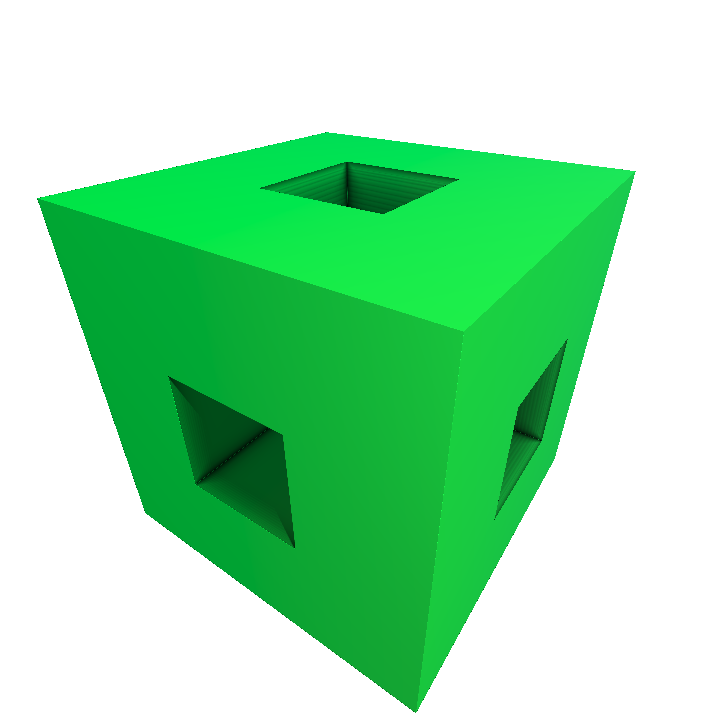
\includegraphics[width=\textwidth]{mengersponge1.png}
        \caption{}
        \label{fig:menger:sponge1}
    \end{subfigure}
    \hfill
    \begin{subfigure}[t]{0.11\textwidth}
        \centering
        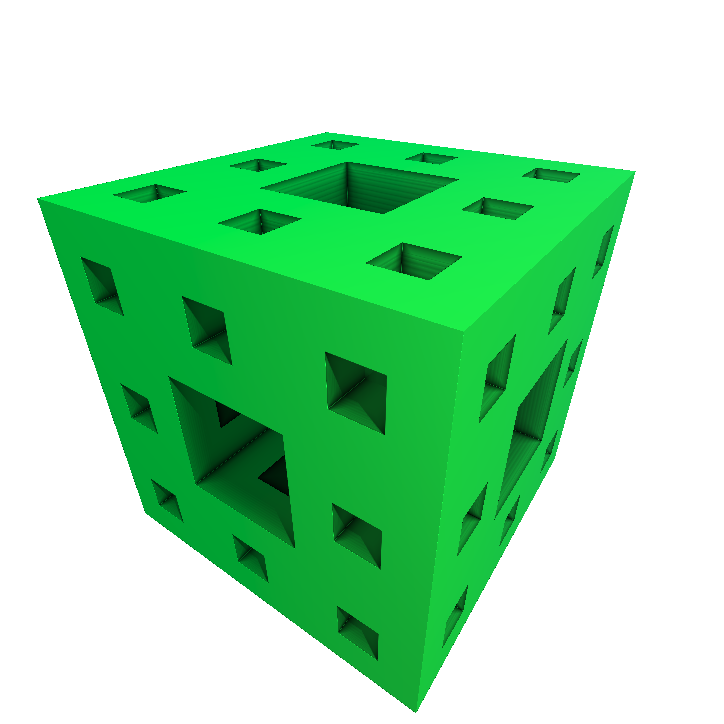
\includegraphics[width=\textwidth]{mengersponge2.png}
        \caption{}
        \label{fig:menger:sponge2}
    \end{subfigure}
    \hfill
    \begin{subfigure}[t]{0.11\textwidth}
        \centering
        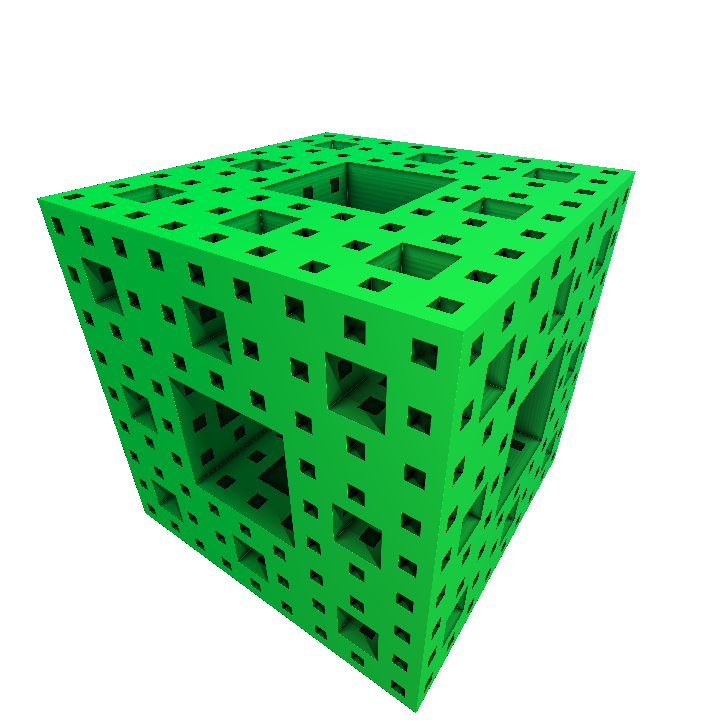
\includegraphics[width=\textwidth]{mengersponge3.png}
        \caption{}
        \label{fig:menger:sponge3}
    \end{subfigure}
    \begin{subfigure}[t]{0.11\textwidth}
        \centering
        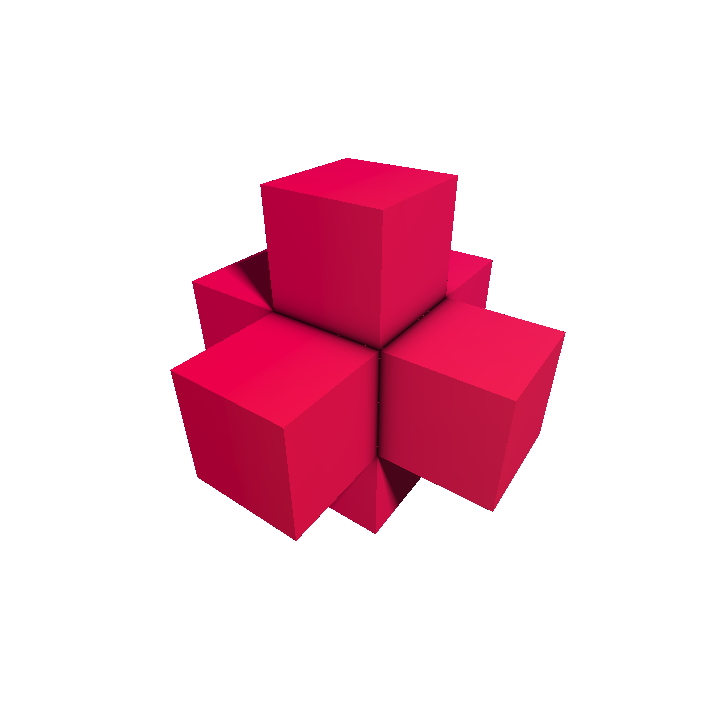
\includegraphics[width=\textwidth]{mengercross0.png}
        \caption{}
        \label{fig:menger:cross0}
    \end{subfigure}
    \hfill
    \begin{subfigure}[t]{0.11\textwidth}
        \centering
        
\includegraphics[width=\textwidth]{mengercross1.png}
        \caption{}
        \label{fig:menger:cross1}
    \end{subfigure}
    \hfill
    \begin{subfigure}[t]{0.11\textwidth}
        \centering
        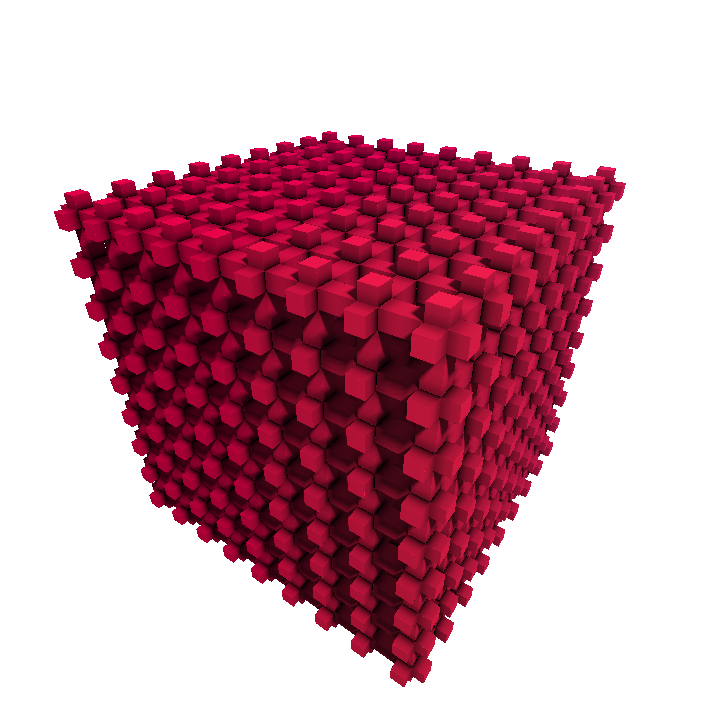
\includegraphics[width=\textwidth]{mengercross2.png}
        \caption{}
        \label{fig:menger:cross2}
    \end{subfigure}
    \begin{subfigure}[t]{0.11\textwidth}
        % subfigure used for alignment
        \centering
        
\includegraphics[width=\textwidth]{placeholder.png}
    \end{subfigure}
    \caption{Iterativ entstehender Menger-Sponge.}
    \label{fig:menger}
\end{figure}

\subsection{Interaktion mit dem Lenia-Mesh}
Der in Kapitel \ref{sec:lenia} besprochene Lenia-Algorithmus kann auf Mesh-Oberflächen angewendet werden.
Das in diesem Kapitel vorgestellte Ray-Marching-Verfahren stellt jedoch keine Mesh-Objekte dar.
Das in \autoref{fig:ray_and_mesh} gezeigte Ergebnis ergibt sich dadurch, dass es einen Shader für das Ray-Marching und einen für das Mesh-Objekt gibt.
Mit dem Ray-Marching-Shader kann eine Environment-Map erzeugt werden, die im Mesh-Shader für die Reflexionen verwendet wird.
Wenn der Depth-Buffer beider Fragment-Shader entsprechend angepasst wird, ist es auch möglich, dass ein Objekt aus dem einen Shader das Objekt aus dem anderen Shader verdeckt.
Auf die bei der Implementierung zu beachtenden Details wird in diesem Bericht nicht weiter eingegangen.

\begin{figure}[!htbp]\centering
    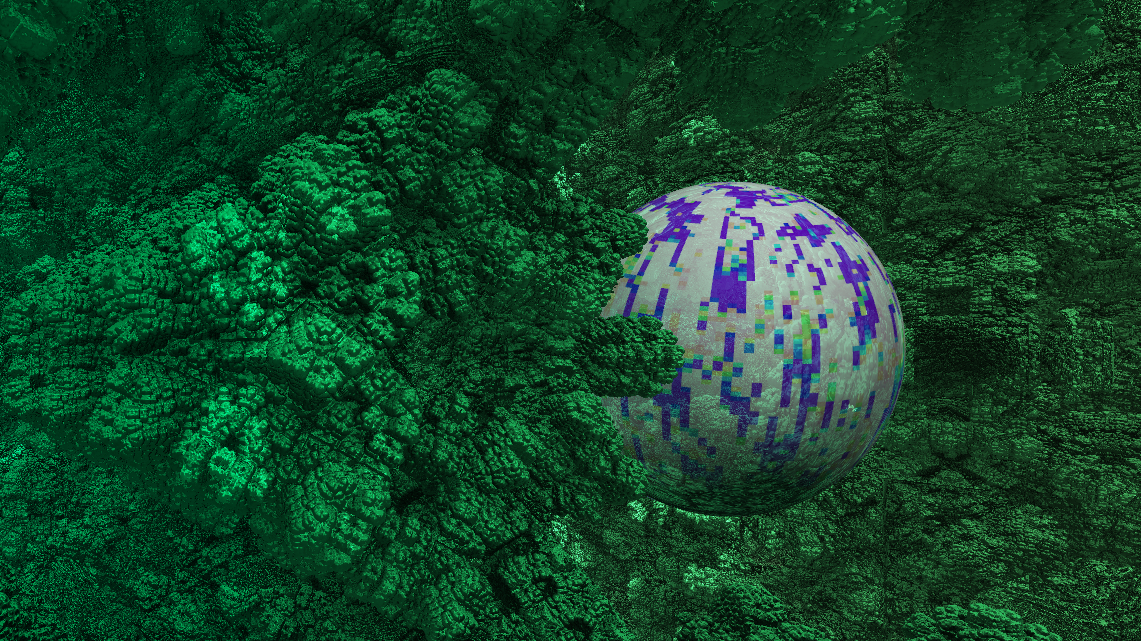
\includegraphics[width=0.5\textwidth - 7.82454pt]{overlap_cropped_bright.png}
    \caption{Überschneidung von Mesh-Objekt mit Ray-Marching Objekt und Reflexion.}
    \label{fig:ray_and_mesh}
\end{figure}


\section{Fazit}
Zusammenfassend lässt sich sagen, dass die vorgestellten Methoden vielfältige Möglichkeiten bieten, um von der Biologie inspirierte Visualisierungen zu erzeugen und dabei weiterhin Raum für kreative Ideen lassen.
Die vorgestellten Algorithmen laufen auf entsprechend leistungsfähiger Hardware in Echtzeit und können durch Veränderung der Parameter in Echtzeit angepasst werden.


%------------------------------------------------

% \section{Methods}

% \begin{figure*}[ht]\centering % Using \begin{figure*} makes the figure take up the entire width of the page
% 	\includegraphics[width=\linewidth]{view}
% 	\caption{Wide Picture}
% 	\label{fig:view}
% \end{figure*}

% \lipsum[4] % Dummy text

% \begin{equation}
% 	\cos^3 \theta =\frac{1}{4}\cos\theta+\frac{3}{4}\cos 3\theta
% 	\label{eq:refname2}
% \end{equation}

% \lipsum[5] % Dummy text

% \begin{enumerate}[noitemsep] % [noitemsep] removes whitespace between the items for a compact look
% 	\item First item in a list
% 	\item Second item in a list
% 	\item Third item in a list
% \end{enumerate}

% \subsection{Subsection}

% \lipsum[6] % Dummy text

% \paragraph{Paragraph} \lipsum[7] % Dummy text
% \paragraph{Paragraph} \lipsum[8] % Dummy text

% \subsection{Subsection}

% \lipsum[9] % Dummy text

% \begin{figure}[ht]\centering
% 	\includegraphics[width=\linewidth]{results}
% 	\caption{In-text Picture}
% 	\label{fig:results}
% \end{figure}

% Reference to Figure \ref{fig:results}.

% %------------------------------------------------

% \section{Results and Discussion}

% \lipsum[10] % Dummy text

% \subsection{Subsection}

% \lipsum[11] % Dummy text

% \begin{table}[hbt]
% 	\caption{Table of Grades}
% 	\centering
% 	\begin{tabular}{llr}
% 		\toprule
% 		\multicolumn{2}{c}{Name} \\
% 		\cmidrule(r){1-2}
% 		First name & Last Name & Grade \\
% 		\midrule
% 		John & Doe & $7.5$ \\
% 		Richard & Miles & $2$ \\
% 		\bottomrule
% 	\end{tabular}
% 	\label{tab:label}
% \end{table}

% \subsubsection{Subsubsection}

% \lipsum[12] % Dummy text

% \begin{description}
% 	\item[Word] Definition
% 	\item[Concept] Explanation
% 	\item[Idea] Text
% \end{description}

% \subsubsection{Subsubsection}

% \lipsum[13] % Dummy text

% \begin{itemize}[noitemsep] % [noitemsep] removes whitespace between the items for a compact look
% 	\item First item in a list
% 	\item Second item in a list
% 	\item Third item in a list
% \end{itemize}

% \subsubsection{Subsubsection}

% \lipsum[14] % Dummy text

% \subsection{Subsection}

% \lipsum[15-23] % Dummy text

% %------------------------------------------------

% \phantomsection
% \section*{Acknowledgments} % The \section*{} command stops section numbering

% \addcontentsline{toc}{section}{Acknowledgments} % Adds this section to the table of contents

% So long and thanks for all the fish \cite{Figueredo:2009dg, Smith:2012qr}.

%----------------------------------------------------------------------------------------
%	REFERENCE LIST
%----------------------------------------------------------------------------------------

\phantomsection
% \bibliographystyle{unsrt}
% \bibliography{sample.bib}
\printbibliography

%----------------------------------------------------------------------------------------

\end{document}